\documentclass[12pt,aspectratio=169]{beamer}

\usetheme[progressbar=frametitle, numbering=fraction]{metropolis}
\usepackage{appendixnumberbeamer}
\usepackage{gensymb}
\usepackage{booktabs}
\usepackage[scale=2]{ccicons}

\usepackage{pgfplots}
\usepgfplotslibrary{dateplot}
\usepackage[english]{babel}

\usepackage{xspace}
\newcommand{\themename}{\textbf{\textsc{metropolis}}\xspace}

% Chinese Fonts (Fontset: fandol,ubuntu)
\usepackage[fontset=windows]{ctex}

% Math Fonts
\usefonttheme{professionalfonts} 
\usepackage{mathspec}
\setsansfont[BoldFont={Fira Sans},
Numbers={OldStyle}]{Fira Sans Light}
\setmathsfont(Digits)[Numbers={Lining, Proportional}]{Fira Sans Light}

% Change Color of the theme
\usepackage{xcolor}
\definecolor{DarkGrey}{HTML}{353535}
\definecolor{ECNURed}{RGB}{164,31,53}
\definecolor{ECNUBrown}{RGB}{134,117,77}
\definecolor{BackGround}{RGB}{250,250,250}
\definecolor{MyBlue}{RGB}{0,161,233}
\definecolor{MyRed}{RGB}{228,0,127}
\setbeamercolor{normal text}{ fg= DarkGrey  }
\setbeamercolor{alerted text}{ fg= ECNURed  }
\setbeamercolor{example text}{ fg= ECNUBrown  }

% Bolder Fonts for presenting in a large room 
\setsansfont[BoldFont={Fira Sans SemiBold}]{Fira Sans}
\metroset{block=fill}

\usepackage{listings,xcolor}
\usepackage{tikz}
\usepackage{pgfmath}
\usepackage{animate,media9,graphicx}
\usepackage{calligra}
\usepackage{array}
\renewcommand{\arraystretch}{2}  % 增加行高
\setlength{\tabcolsep}{10pt}       % 增加列间距

\lstset{
	language         = c++,
	numbers          = left,
	numberstyle      = \tiny,
	breaklines       = true,
	captionpos       = b,
	tabsize          = 4,
	frame            = shadowbox,
	columns          = fullflexible,
	commentstyle     = \color[RGB]{0,128,0},
	keywordstyle     = \color[RGB]{0,0,255},
	basicstyle       = \tiny\ttfamily,
	stringstyle      = \color[RGB]{148,0,209}\ttfamily,
	rulesepcolor     = \color{red!20!green!20!blue!20},
	showstringspaces = false,
}

\title{PathFormer}
\subtitle{Multi-scale Transformers with Adaptive Pathways for Time Series Forecasting}
\date{\today}
\author{Yifei Ding}
% \institute{演讲者描述}
% \titlegraphic{\hfill
\includegraphics[height=1.5cm]{ECNUlogo.png}}

\begin{document}

\maketitle
% \footnotesize
\begin{frame}{Contents}
  \setbeamertemplate{section in toc}[sections numbered]
  \tableofcontents%[hideallsubsections]
\end{frame}


\section{Introduction}

\begin{frame}{Introduction}

  Motivations:

  \begin{itemize}

  	\item Transformer calls for better designs and adaptations to fulfill 
    its potential.
  
  	\item Temporal resolution and temporal distance need to be considered.

  \end{itemize}

  Challengs:

  \begin{itemize}

	\item \textit{Incompleteness of multi-scale modeling};
	\item \textit{Fixed multi-scale modeling}.

  \end{itemize}

\end{frame}

\section{Related Work}

\begin{frame}{Related Work}

  Time series forecasting:

  \begin{itemize}

    \item Deep learning methods: GNNs, RNNs, DeepAR, CNN, TimesNet, 
    LLM-based methods, etc.
    \item Transformer models: Informer, Triformer, Autoformer, FEDformer, 
    PatchTST, etc.

  \end{itemize}

  Multi-scale modeling for time series:

  \begin{itemize}

    \item N-HiTS, Pyraformer, Scaleformer, etc.

  \end{itemize}

\end{frame}

\section{Methodology}

\begin{frame}{Methodology}

  \begin{figure}

    \centering
    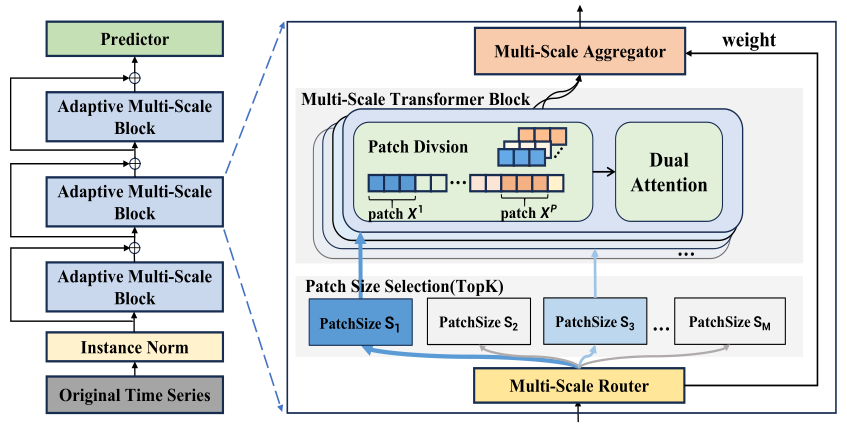
\includegraphics[width=0.8\textwidth]{fig/framework.png}
    \caption{The Architecture of PathFormer.}

  \end{figure}

\end{frame}

\subsection{Multi-scale Transformer Block}

\begin{frame}{Multi-scale Transformer Block}

  \begin{figure}

    \centering
    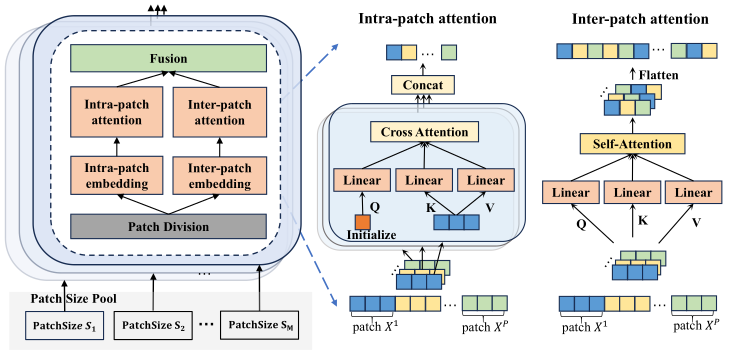
\includegraphics[width=0.8\textwidth]{fig/multi-scale transformer block.png}
    \caption{Multi-scale Transformer Block.}

  \end{figure}

\end{frame}

\begin{frame}{Multi-scale Transformer Block}

  \textbf{1.Multi-scale Division.}

  \begin{itemize}

    \item Define a collection of $M$ patch size values as 
    ${\cal S}=\{S_1,S_2,\cdots,S_M\}$;
    \item Define the input time series as $X\in\mathbb{R}^{H\times d}$, 
    where $H$ represents the length of the time series and $d$ represents 
    the dimension of features.

  \end{itemize}

  For each $i\in[1,M]$, divide $X$ into ${\color{ECNURed}(X^1,X^2,\cdots,X^{P_i})},
  P_i=H/S_i,X^j\in\mathbb{R}^{S_i\times d},\allowbreak j\in[1,P_i]$.

\end{frame}

\begin{frame}{Multi-scale Transformer Block}

  \textbf{2.Dual Attantion.}

  \textit{\color{ECNURed}{Intra-patch Attantion}:}

  \begin{itemize}

    \item Embed the patchs along the feature dimension $d$ to get 
    $X_\mathrm{intra}^j\in\mathbb{R}^{S_i\times d_m},\allowbreak\forall j\in[1,P_i]$;
  
    \item Perform trainable linear transformations on $X_\mathrm{intra}^j$ to get 
    $K_\mathrm{intra}^j,V_\mathrm{intra}^j\in\mathbb{R}^{S_i\times d_m}$;
  
    \item Employ a trainable query matrix 
    $Q_\mathrm{intra}^j\in\mathbb{R}^{1\times d_m}$.

  \end{itemize}

  \vspace{-0.5cm}
  
  $$\mathrm{Attn}_\mathrm{intra}^j=\mathrm{Softmax}\left(Q_\mathrm{intra}^j(K_\mathrm{intra}^j)^T/\sqrt{d_m}\right)V_\mathrm{intra}^j,$$

  \vspace{-0.5cm}

  {\color{ECNURed}

    $$\mathrm{Attn}_\mathrm{intra}=\mathrm{Concat}\left(\mathrm{Attn}_\mathrm{intra}^1,\cdots,\mathrm{Attn}_\mathrm{intra}^{P_i}\right).$$
  
  }

\end{frame}

\begin{frame}{Multi-scale Transformer Block}

  \textbf{2.Dual Attantion.}

  \textit{\color{ECNURed}{Inter-patch Attantion:}}

  \begin{itemize}

    \item Embed feature along the feature dimension $d$ to $d_m$;

    \item Rearrange the data to combine the two dimensions of $S_i$ and $d_m$,
    making $X_\mathrm{inter}\in\mathbb{R}^{P_i\times d_m'}, d_m'=S_i\cdot d_m$;

    \item Obtain $Q_\mathrm{inter},K_\mathrm{inter},V_\mathrm{inter}\in
    \mathbb{R}^{P_i\times d_m'}$ by linear mapping on $X_\mathrm{inter}$.

  \end{itemize}

  \vspace{-0.5cm}

  {\color{ECNURed}

    $$\mathrm{Attn}_\mathrm{inter}=\mathrm{Softmax}\left(Q_\mathrm{inter}(K_\mathrm{inter})^T/\sqrt{d_m'}\right)V_\mathrm{inter}.$$
    
  }

\end{frame}

\begin{frame}{Multi-scale Transformer Block}

  \textbf{2.Dual Attantion.}

  \textit{Final Output of Dual Attantion:}

  \begin{itemize}

    \item Rearrange the outputs of intra-patch attantion to 
    $\mathrm{Attn}_\mathrm{intra}\in\mathbb{R}^{P_i\times S_i\times d_m}$ by 
    performing linear transformations on the patch size dimension from $1$ to $S_i$;

    \item Add $\mathrm{Attn}_\mathrm{intra}$ with $\mathrm{Attn}_\mathrm{inter}
    \in\mathbb{R}^{P_i\times S_i\times d_m}$ to obtain the final output of 
    dual attantion {\color{ECNURed}$\mathrm{Attn}\in\mathbb{R}^{P_i\times S_i\times d_m}$}.

  \end{itemize}

\end{frame}

\subsection{Adaptive Pathways}

\begin{frame}{Adaptive Pathways}

  \begin{figure}

    \centering
    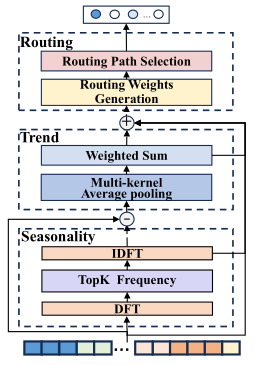
\includegraphics[width=0.3\textwidth]{fig/multi-scale router.png}
    \caption{Multi-scale Router.}

  \end{figure}

\end{frame}

\begin{frame}{Adaptive Pathways}

  \textbf{1.Multi-scale Router.}

  \textit{\color{ECNURed}Seasonality Decomposition:}

  \begin{itemize}

    \item Utilize DFT to decompose $X$ into Fourier basis;
    \item Select the $K_f$ basis with the largest amplitudes;
    \item Obtain {
      \color{ECNURed}
      $X_\mathrm{sea}=\mathrm{IDFT}\left(\{f_1,f_2,\cdots,f_{K_f}\},A,\Phi\right)$
    }, where $\Phi$ and $A$ represent the phase and amplitude of each frequency
    from $\mathrm{DFT}(X)$, $\{f_1,f_2,\cdots,f_{K_f}\}$ represent the frequencies 
    with top $K_f$ amplitudes.

  \end{itemize}

\end{frame}

\begin{frame}{Adaptive Pathways}

  \textbf{1.Multi-scale Router.}

  \textit{\color{ECNURed}Trend Decomposition:}

  \begin{itemize}

    \item Get the remaining part after the seasonality decomposition
    $X_\mathrm{rem}=X-X_\mathrm{sea}$;

    \item Obtain the result from average poolings with different kernels and a 
    weighted operation:
  \end{itemize}
  {\color{ECNURed}
    $$X_\mathrm{trend}=\mathrm{Softmax}(L(X_\mathrm{rem}))
    \cdot(\mathrm{Avgpool}_{\mathrm{kernel}_1}(X_\mathrm{rem}),\cdots,
    \mathrm{Avgpool}_{\mathrm{kernel}_N}(X_\mathrm{rem}));$$}
\end{frame}

\begin{frame}{Adaptive Pathways}

  \textbf{1.Multi-scale Router.}

  \textit{Final Result of Multi-scale Router:}

  \begin{itemize}

    \item Add $X_\mathrm{sea},X_\mathrm{trend}$ with $X$ and
    perform a linear mapping $\mathrm{Linear}(\cdot)$ to transform and merge
    them along the temporal dimension to get $X_\mathrm{trans}\in\mathbb{R}^{d}.$

    \item Generate pathway weights:

  \end{itemize}

  \vspace{-0.7cm}

  $$R(X_\mathrm{trans})=\mathrm{Softmax}
  (X_\mathrm{trans}W_r+\varepsilon\cdot\mathrm{Softplus}
  (X_\mathrm{trans}W_\mathrm{noise})),\varepsilon\sim{\cal N}(0,1);$$

  \begin{itemize}

    \item Perform top$K$ selection on the pathway weights, keeping the top $K$ 
    pathway weights and setting the rest weights as $0$, and denote the final
    result as {\color{ECNURed}$\overline{R}(X_\mathrm{trans}).$}

  \end{itemize}

\end{frame}

\begin{frame}{Adaptive Pathways}

  \textbf{2.Multi-scale Aggregator.}

  \begin{itemize}

    \item Let $X_\mathrm{out}^i$ denote the output of the multi-scale Transformer
    with the patch size $S_i$;

    \item Define $T_i(\cdot)$ as a transformation function to align the temporal 
    dimension from different scales;

    \item Get the final output of AMS block:

  \end{itemize}

  \vspace{-0.7cm}

  {

    \color{ECNURed}
    $$X_\mathrm{out}=\sum_{i=1}^M {\cal I}\left(\overline{R}
    \left(X_\mathrm{trans}\right)_i>0\right)R(X_\mathrm{trans})_i
    T_i(X_\mathrm{out}^i).$$

  }

\end{frame}

\section{Experiments}

\begin{frame}{Experiments}

  \textbf{Time Series Forecasting:}

  \begin{itemize}

    \item The best performance in 81 cases and the second-best performance in 5
    cases out of the overall 88 cases;

    \item Demonstrate a significant improvement when compared with PatchTST;

    \item Outperform when compared with strong linear models NLinear.

  \end{itemize}

  \textbf{Transfer Learning:}

  \begin{itemize}

    \item Can provide effictive lightweight transfer learning for time series 
    forecasting.

  \end{itemize}

\end{frame}

\begin{frame}{Experiments}

  \textbf{Ablation Studies:}

  \begin{itemize}

    \item Verying the Number of Adaptively Selected Patch Sizes:

    \begin{itemize}

      \item Adaptively modeling critical multi-scale characteristics improves 
      accuracy;

      \item Distinct time series samples benefit from feature extraction using 
      varied patch sizes, but not all patch sizes are equally effictive.

    \end{itemize}

    \item Visualization of Pathways Weights:

    \begin{itemize}

      \item Underscore PathFormer's adaptability, emphasizing its ability to
      discern and apply the optimal patch size combinations for the diverse
      seasonality and trend patterns across samples.

    \end{itemize}

  \end{itemize}

\end{frame}

\begin{frame}{Acknowledgement}

  \begin{center}

    \textcolor{gray}{\Huge{\centerline{\calligra{Thank you!}}}}

  \end{center}

\end{frame}

\end{document}